\chapter{Static Single Information Form \Author{F. Pereira}}
\inputprogress
\label{chap:ssi}

\graphicspath{{img/}{ssi/img/}{part2/ssi/img/}}

\section{Introduction}
\label{sec:ssi:pereira:intro}

The objective of a dataflow analysis is to discover facts that are true about a
program.
We call such facts {\em informations}.
Using the notation introduced in Section~\ref{novillo:sec:property_space}, an
information is a point in the dataflow lattice.
For example, liveness analysis is interested in finding out the set of
variables alive at a certain program point.
Similarly to liveness analysis, many other classic dataflow approaches bind
information to pairs formed by a variable and a program point.
However, if the information is true for a variable $v$ at any program point where
$v$ is alive, then we can associate this information directly to $v$.
If a program's intermediate representation guarantees this correspondence between
information and variable for every variable, then we say that the program
representation provides the {\em Single Static Information} (SSI) property.

Different dataflow analysis might extract information from different program
facts.
Therefore, a program representation may afford the SSI property to some dataflow
analysis, but not to all of them.
For instance, the SSA form naturally provides the SSI property to the reaching
definition analysis.
Indeed, the SSA form provides the static single information property to any
dataflow analysis that obtains information at the definition sites of
variables.
These analyses and transformations include classic constant propagation, as
seen in Chapter~\ref{chap:constant_propagation_is_easier}, and simple versions of
type inference, for instance.
However, the SSA form does not provide the SSI property to a dataflow analysis
that derives information from the use site of variables.
In other words, because the same variable $v$ in a SSA form program might be used
at different program points, the informations associated to $v$ might not be
unique.

There exist extensions of the SSA form that provide the SSI property to more
dataflow analyses than the original SSA does.
Two classic examples are the {\em Extended-SSA} (e-SSA) form introduced by Bodik
{\em et al.}~\cite{Bodik00}, and the {\em Static Single Information} (SSI) form
introduced by Ananian~\cite{Ananian99}.
The e-SSA form provides the SSI property to analyses that take information from
the definition site of variables, and also from conditional tests where these
variables are used.
Ananian's SSI form gives the static single information property to dataflow
analyses that extract information from particular use sites of variables, such
as {\em Busy Expressions Analysis}.
A common strategy that any of these intermediate representations use to achieve
the SSI property is {\em live range splitting}.
In this chapter we show how to use live range splitting to build program
representations that provide the static single information property to different
types of dataflow analysis.

\section{Live Range Splitting}
\label{sec:ssi:pereira:split}

A program representation that splits the live range of each variable between each
pair of consecutive program points naturally provides the SSI property to any
dataflow analysis that discovers facts about variables.
Actually, such a program representation exists: it is called {\em elementary
form}, and it has even seen use in optimizations such as register
allocation~\cite{Appel01,Pereira08}.
However, this strategy lends to the dataflow analysis many identity transfer
functions.
For instance, in liveness analysis, an instruction that does not use nor define
any variable is bound to an identity transfer function: it simply propagates the
values that come from its successors to its predecessors.
Therefore, we would like to split the live ranges of variables only at program
points where information about that variable is produced.

We call a {\em generator} a program point that produce information about a
variable.
A generator is usually an instruction, such as a use or a definition of a
variable in our liveness analysis example.
However, generators can also be conditional branches or even the entry/exit
nodes of the program's control flow graph (CFG).
Some program points are considered {\em meet nodes}, because they combine the
information that comes from two or more regions.
If a program point represents a meet node, then we call it a
{\em combinator}.
Ideally, we would like to split the live ranges of variables only at program
points which are either generators or combinators.

\subsection{Special instructions to split live ranges}
\label{sub:ssi:instructions}

We split the live range of a variable $v$ at program point $p$ in a two steps
process.
Firstly, we insert a copy $v' = v$ at $p$.
Secondly, we rename to $v'$ every use of $v$ at any program point $p'$ dominated
by $p$.
After performing the renaming phase, we might have to insert $\phi$-functions in
the source program in order to avoid having two different denotations of the
same variable alive together.

In principle we could split the live ranges of many variables at the same
program point using simple copies; however, this notation brings semantic
complications: which variable was created first? Which variables are alive
together?
In order to avoid such questions, we use special instructions to perform
live range splitting.
There exists three basic types of program points where we might split live
ranges: interior nodes, branches and joins.
At each place we use a different notation to represent live range splitting.

% need phi
We call {\em joins} the program points that have one successor and
multiple predecessors.
Notice that because each program point exists before or after a program
instruction, there exist no program point with multiple predecessors and
successors.
We split live ranges at join nodes via $\phi$-functions.
Therefore, the SSA form already suits dataflow analysis that combine information
at these nodes.

% Interior nodes
{\em Interior nodes} are program points that have a unique predecessor and a
unique successor.
At these points we perform live range splitting via parallel copies.
A parallel copy such as:
\[
(v_1, \ldots, v_n) = (v_1', \ldots, v_n')
\]
performs $n$ assignments like $v_i = v_i'$; all in parallel.
These copies are used mostly by dataflow analysis that generate information
from the uses of variables.
As a first example, lets consider the backward analysis used by An
{\em et al.} to type Ruby programs~\cite{An11}.
The set of infered types of a variable $v$ might be different before and after
a use point $p$ where $v$ is used.
For instance, if we have a use of $v$ such as $v.m()$, then we know, from this
point backwards, that $v$ must have the method $m$.
We should split the live range of $v$ at $p$ by inserting a copy $(v')=(v)$ at
that point, where $v'$ is a fresh name.

% need sigma
A {\em branch point}, is a program point with a unique predecessor and multiple
successors.
Going back to An's type inference engine~\cite{An11}, we may have that the
definition of a variable $v$ feeds two uses of this variable, e.g, $v.m_1()$
and $v.m_2()$, through different program paths.
We would like to infer that $v$ contains both methods, $m_1()$ and $m_2()$.
Put in another way, the use that reaches the definition of $v$ must be unique,
in the same way that in a SSA-form program the definition that reaches a use
is unique.
We ensure this uniqueness via another type of special instructions: the
$\sigma$-functions.
Consider, for instance, the assignment below:
\[
[(v_{11}, \ldots, v_{n1}):l_1, \ldots (v_{1m}, \ldots, v_{nm}):l_m] =
 \sigma(v_1, \ldots, v_n)
\]
which represents $n$ $\sigma$-nodes such as
$(v_{i1}:l_1, \ldots, v_{im}:l_m) \leftarrow \sigma (v_i)$.
This instruction assigns to each variable $v_{ij}:l_j$ the
value in $v_i$ if control flows into block $l_j$.
These assignments happen in parallel, i.e., these $n$
$\sigma$-functions encapsulate $m$ parallel copies.
Also, notice that variables alive in different branches of a basic block are
given different names by the $\sigma$-function that ends that basic block.

There is a beautiful symmetry between $\phi$- and $\sigma$-functions.
Whereas the latter has the functionality of a variable multiplexer, the former
is analogous to a demultiplexer, that performs a parallel assignment depending
on the execution path taken.
To see this duality more clearly, we can represent a $\phi$-function as a
set of $m$ parallel copies:
\[
(v_1, \ldots, v_n) = \phi[(v_{11}, \ldots, v_{n1}):l_1, \ldots (v_{1m}, \ldots,
v_{nm}):l_m]
\]
The assignment above contains $n$ $\phi$-functions such as
$v_i \leftarrow \phi(v_{i1}:l_1, \ldots, v_{im}:l_m)$.
It will assign to each $v_i$ the value in $v_{ij}$, where $j$ is determined by
$l_j$, the basic block last visited  before reaching the $\phi$ assignment.
Notice that, just like in the case of $\sigma$-functions, these assignments
happen in parallel.

\subsection{Examples of Live Range Splitting}
\label{sub:ssi:examples}

In order to ensure the static single information property, different dataflow
analysis do live range splitting in different ways.
In this section we will see some meaningful examples.

\paragraph{Points-to analysis}
Points-to analysis computes an approximation of the set of memory locations that
can be pointed-to by a given variable.
In this case, information is extracted from the definition sites of
variables.
Thus, the SSA form already gives to alias analysis the static single property,
as we illustrate in Figure~\ref{fig:aliasAnalysis}.
Figure~\ref{fig:aliasAnalysis}(a) shows the control flow graph of an 
example program, and Figure~\ref{fig:aliasAnalysis}(b) shows the same CFG,
this time in SSA form.
Notice that we have augmented instructions with labels, which we will use later
to explain where to split live ranges.
The SSA graph of this program, as discussed in Chapter~\ref{chap:vsdg}, is given
in Figure~\ref{fig:aliasAnalysis}(c).
If we represent by $I$ the information bound to each variable, then from our
program representation we derive the constraint system shown
Figure~\ref{fig:aliasAnalysis}(d)
A fix-point to this constraint system is a solution to our dataflow problem.
Notice that the solution of this dataflow problems depends only on the
inter-relations between the program variables.
As we will see in the rest of this section, this is a common characteristics of
dataflow analyses that bind information to the live ranges of variables.


\begin{figure}[t!]
\centering
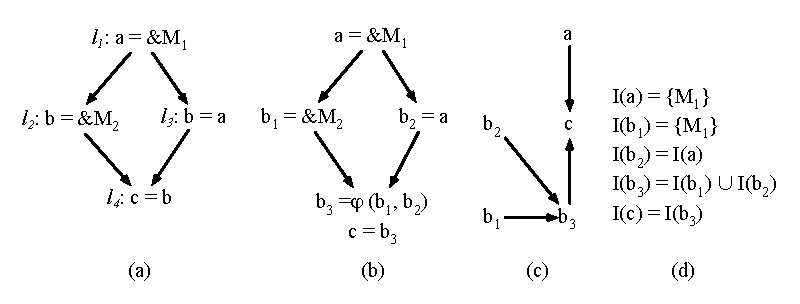
\includegraphics[width=\linewidth]{aliasAnalysis}
\caption{Alias analysis as an example of forward dataflow analysis that takes information from the definition of variables.}
\label{fig:aliasAnalysis}
\end{figure}


\paragraph{Type Inference}
A type inference engine learns information from the uses of a variable, and
tries to assign a principal type to this variable's definition, in such a way
that the program would be semantically correct.
Lets illustrates an instance of type inference using the Python program in
Figure~\ref{fig:typeInference}(a).
Our objective is to infer the correct suite of methods for each object bound to
variable $v$.
Figure~\ref{fig:typeInference}(b) shows the control flow graph of the
program, and Figure~\ref{fig:typeInference}(c) shows the methods inferred to
variable $v$ at each program point.
Some instructions, such as that in label $l_3$, have no influence on these sets.
On the other hand, instructions like those at $l_4$, $l_6$ or $l_7$ let
us infer methods that belong into $v$.
Similarly, the instructions at $l_1$ and $l_5$ kill the information that comes
from their predecessors.
All these instructions generate some sort of information to the type inference
engine.
Finally, the instruction at $l_2$ combines the possibly different informations
that flow back from the two program paths that originate at it.
These six program points are bound to non-identity transfer functions, in the
context of the type inference analysis.
If we split the live range of $v$ at these program points, then we get the
program representation given in Figure~\ref{fig:typeInference}(d).
We do not need to split $v$'s live range neither at $l_1$ nor at $l_5$, because
$v$ is not alive before these points.
Notice that the $\phi$-function at $l_7$ only exists because we want to
stay in SSA-form; hence, it joins the names created due to live range splitting.
The constraints that characterize this dataflow program are given in
Figure~\ref{fig:typeInference}(e).

\begin{figure}[t!]
\centering
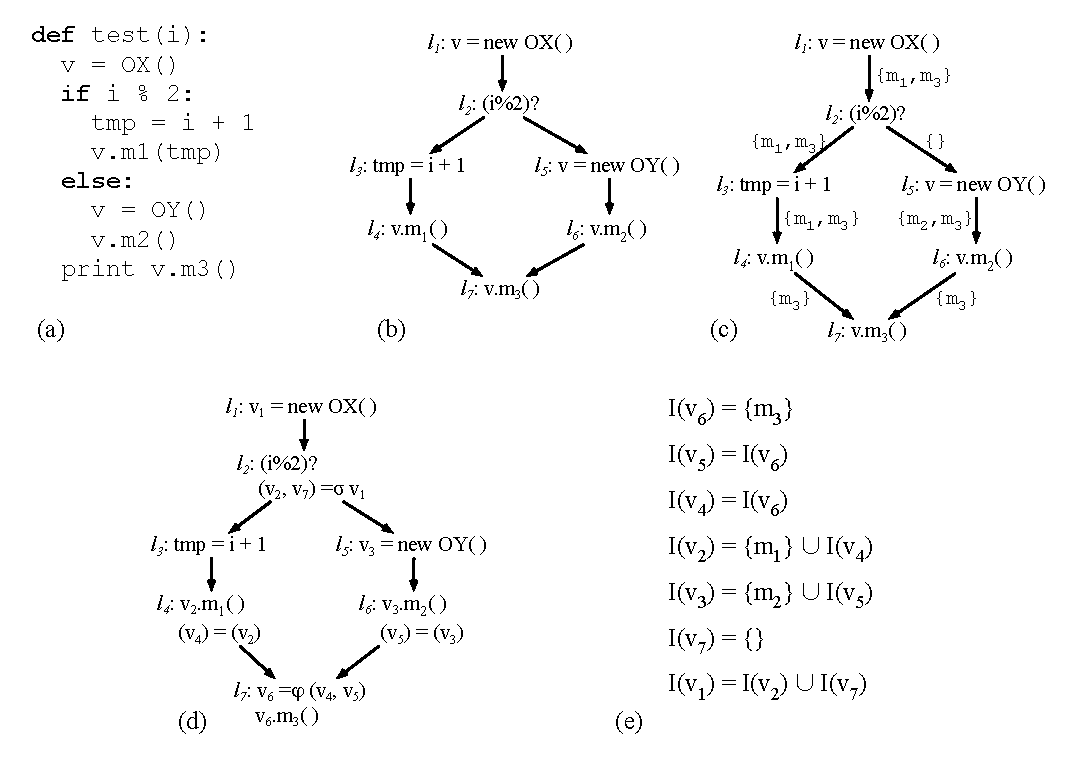
\includegraphics[width=\linewidth]{fullEx}
\caption{Type inference analysis as an example of backward dataflow analysis
that takes information from the uses of variables.}
\label{fig:typeInference}
\end{figure}

\paragraph{Taint analysis}
The objective of taint analysis~\cite{Rimsa11} is to find program
vulnerabilities.
In this case, a harmful attack is possible when input data reaches sensitive
program sites without going through special functions called sanitizers.
Figure~\ref{fig:taintAnalysis} illustrates this type of analysis.
We have used $\phi$ and $\sigma$-functions to split the live ranges of the
variables in Figure~\ref{fig:taintAnalysis}(a) producing the program in
Figure~\ref{fig:taintAnalysis}(b).
This intermediate representation, called {\em Extended Static Single
Assignment} (e-SSA) form, is the same introduced by Bodik
{\em et al.}~\cite{Bodik00} to remove redundant array bound checks.

Lets assume that {\em echo} is a sensitive function, because it is used to
generate web pages.
For instance, if the data passed to {\em echo} is a JavaScript program, then
we could have an instance of cross-site scripting attack.
Therefore, from this last figure we know that the instruction
$\mathit{echo} \ v_1$ is a source of vulnerabilities, as it outputs data that
comes directly from the program input.
On the other hand, we know that $\mathit{echo} \ v_2$ is always safe, for
variable $v_2$ is initialized with a constant value.
We can use specific functions, the {\em sanitizers}, to clean data, or to
check that data is safe.
The call $\mathit{echo} \ v_5$ is always safe, because the variable $v_5$
has been sanitized; however, the call $\mathit{echo} \ v_4$ might be
tainted, as variable $v_4$ results from a failed attempt to sanitize $v$.
The SSA graph is given in Figure~\ref{fig:taintAnalysis}(c), and the
corresponding constraints are shown in Figure~\ref{fig:taintAnalysis}(d).

\begin{figure}[t!]
\centering
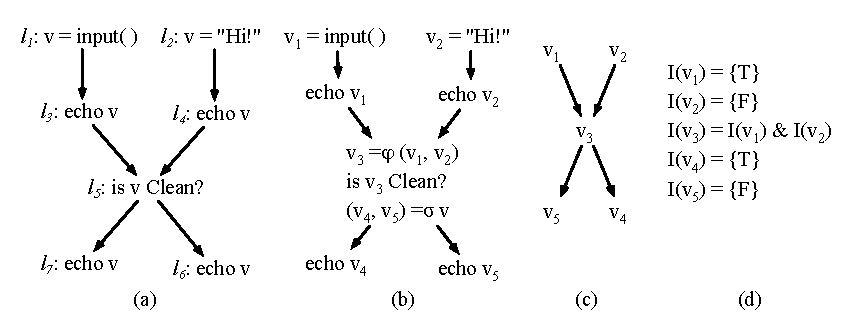
\includegraphics[width=\linewidth]{taintAnalysis}
\caption{Taint analysis as an example of forward dataflow analysis that takes
information from the definitions of variables and conditional tests on these
variables.}
\label{fig:taintAnalysis}
\end{figure}

\paragraph{Null pointer analysis}
The objective of null pointer analysis is to determine which references may
hold null values.
Nanda and Sinha have used a variant of this analysis to find which method
dereferences may throw exceptions, and which may not~\cite{Nanda09}.
This analysis allows compilers to remove redundant null-exception tests and
helps developers to find null pointer dereferences.
Figure~\ref{fig:nullAnalysis} illustrates an example of this analysis.
Because we take information from use sites, in Figure~\ref{fig:nullAnalysis}(b)
we have split the live range of each variable right after it its used.
Thus, we know, for instance, that the call $v_2.m()$ cannot be null, otherwise
an exception would have been thrown during the invocation $v_1.m()$.
On the other hand, in Figure~\ref{fig:nullAnalysis}(c) we notice that the state
of $v_4$ is the meet of the state of $v_3$, definitely not-null, and the state
of $v_1$, possibly null, and we must conservatively assume that $v_4$ may be
null.
Notice that the program representation that we use for a given dataflow problem
depends on the level of detail that we obtain from the source code.
Null pointer checks are implemented as exceptions, which are guarded by
conditional tests.
If we had access to the code of these tests, then we would implement the
null pointer analysis using the same representation that we use for the tainted
flow problem.

\begin{figure}[t!]
\centering
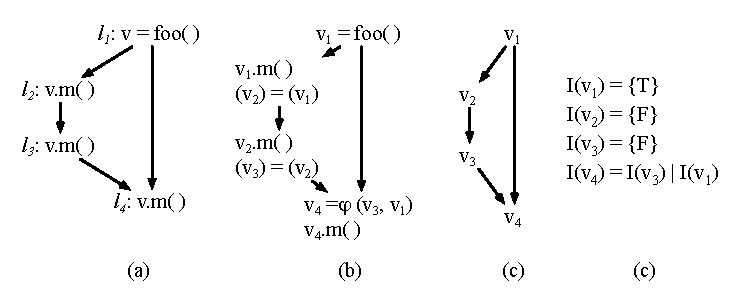
\includegraphics[width=\linewidth]{nullAnalysis}
\caption{Null pointer analysis as an example of forward dataflow analysis that takes information from
the definitions and uses of variables.}
\label{fig:nullAnalysis}
\end{figure}


\section{Live Range Splitting Strategies}
\label{sec:ssi:building}

A {\em live range splitting strategy} over a variable $v$, which we denote by
$S_v$, is a pair $(d, P)$.
The first element, $d \subseteq \{\uparrow, \downarrow\}$, denotes a direction
along which the information flows: it can be forward ($\downarrow$) or backward
($\uparrow$).
The second element, $P$, denotes the set of programs points where
the information is acquired.
Going back to the examples from Section~\ref{sub:ssi:examples}, we have the
following live range splitting directives:
\begin{itemize}
\item Alias analysis is a forward analysis that takes information from the
definition site of variables; thus, for each variable $v$, $N$ is the set of
definition points of $v$.
For instance, in Figure~\ref{fig:nullAnalysis}, we have that
$S_{v} = (\downarrow, \{l_2, l_3\})$.

\item Type inference is a backward analysis that takes information from the
uses of variables; thus, for each variable, $N$ is its set of use sites.
For instance, in Figure~\ref{fig:typeInference}(e), we have that
$S_{v} = (\uparrow, \{l_4, l_6\})$.
Notice that we do not split live ranges at the last use of a variable, because
this variable is not alive henceforth.

\item Taint analysis is a forward analysis that takes information from
definition points, and conditional tests that use variables; thus, we split
live ranges at conditionals.
For instance, in Figure~\ref{fig:taintAnalysis}, we have that
$S_{v} = (\downarrow, \{l_1, l_2, l_5\})$.

\item The null pointer check is a forward
analysis that takes information from definitions and uses.
For instance, in Figure~\ref{fig:nullAnalysis}, we have that
$S_{v} = (\downarrow, \{l_1, l_2, l_3\})$.
\end{itemize}
The list in Figure~\ref{fig:splittingSt} gives further examples of live
range splitting strategies.

\begin{figure}[t!]
\begin{center}
\begin{small}
\renewcommand\arraystretch{1.4}
\begin{tabular}{| c | c |} \hline
{\bf Client} & {\bf Splitting strategy} \\ \hline
Alias analysis, reaching definitions & $(\downarrow, \{\mathit{defs}\})$ \\ \hline
SSI Clients~\cite{Ananian99,Singer06} & $(\downarrow,
\{\mathit{defs}\}), (\uparrow, \{\mathit{uses}_{last}\})$ \\ \hline
Cond. constant propagation~\cite{Wegman91}, ABCD~\cite{Bodik00},
 & $(\downarrow, \{\mathit{defs},
\mathit{conds}\})$ \\
Taint analysis~\cite{Rimsa11}, range analysis~\cite{Su05,Gawlitza09} & \\ \hline
Stephenson's Bitwidth Analysis~\cite{Stephenson00} & $(\downarrow,
\{\mathit{defs}, \mathit{conds}\}), (\uparrow, \{\mathit{uses}\})$  \\ \hline
Mahlke's Bitwidth Analysis~\cite{Mahlke01} & $(\downarrow, \{\mathit{defs}\}),
(\uparrow, \{\mathit{uses}\})$  \\ \hline
An's type inference~\cite{An11} & $(\uparrow, \{\mathit{uses}\})$ \\ \hline
Hochstadt's type inference~\cite{Hochstadt08} &
$(\uparrow, \{\mathit{uses}, \mathit{conds}\})$ \\ \hline
Null-pointer analysis~\cite{Nanda09} & $(\downarrow, \{\mathit{defs},
\mathit{uses}\})$ \\ \hline
\end{tabular}
\end{small}
\caption{Live range splitting strategies for different dataflow analyses.
We use $\mathit{def}$ ($\mathit{use}$) to denote the set of instructions that
define (use) the variable;
$\mathit{cond}$ to denote the set of instructions that apply a conditional
test on a variable; and
$\mathit{use}_{last}$ to denote the set of instructions where a
variable is used, and after which it is no longer alive.}
\label{fig:splittingSt}
\end{center}
\end{figure}

\paragraph{Splitting algorithm for forward analyses}

Given a splitting strategy $S_v = (\downarrow, N)$, we split the live
range of $v$ at every program point in $N$.
Some of these program points, like $l_5$ in Figure~\ref{fig:taintAnalysis}, 
have two or more successors.
We split live ranges at these program points via $\sigma$-functions.
After live range splitting, we might have many sources of information
reaching a common program point.
For instance, in Figure~\ref{fig:aliasAnalysis}(a), the information that flows
forward from $l_2$ and $l_3$ collide at $l_4$.
We use a $\phi$-function to merge these two flows.
In our example, this $\phi$-function defines $b_3$.
The set of program points where the information collide is easily characterized
if we use the notion of join sets introduced in
Chapter~\ref{chap:properties_and_flavours}.
Therefore, the very SSA construction algorithm suffices to split live ranges
to forward dataflow analysis.

\paragraph{Splitting algorithm for backward analyses}

A live range splitting strategy $S_v = (\uparrow, N)$ requires us to merge
information that is propagated backwardly.
For instance, lets assume, in Figure~\ref{fig:typeInference}(a), that we did
not have the instruction at $l_5$.
Thus, we would know from the use of $O$'s instance at $l_4$ that the class
$OY$ contains $m_1$.
Similarly, we know, due to $l_6$, that it also contains $m_2$.
These two informations are equally valid at $l_1$; thus, leading us to conclude
that both methods are defined in the object $v$.
In Figure~\ref{fig:typeInference}(b) we represent this backward merge via the
$\sigma$-function $(v_2, v_7) =\sigma v_1$.

We use the notions of split sets and iterated post
dominance frontier, introduced in Chapter~\ref{chap:properties_and_flavours},
to provide the live range splitting algorithm for backward analyses.
However, if necessary to keep the SSA property, then forward and backward
splitting algorithms are not symmetric, as the latter does not ensure
static single definitions.
Thus, splitting for $S_v = (\uparrow, N)$ demands two steps: first we insert
$\sigma$-functions at $\cal{S}(N)$, and do variable renaming, walking up the
program's post-dominator tree.
This renaming step is symmetric to that used to build the SSA form.
In the second phase we reconstruct the SSA form.
The price to stay under SSA-form is that variables created by $\phi$-functions
might be bound to identity transfer functions.
For instance, in Figure~\ref{fig:typeInference}(b) we learn from the use of
$v_6$ that the class $O$ contains method $m_3$.
Our transfer function passes this information from $v_3$ to $v_4$ and $v_5$
without any change.

\paragraph{Extending information beyond variable's live ranges}

The minimal, non pruned SSA form might be useful to those analyses that require
information outside the live range of the variable that originates this
information, such as partial redundancy elimination. 
A $\phi$-function might represent a value useful in value numbering, even if the
original program did not refer to that value~\ref{Choi91}.
Hence, the decision of pruning $\phi$ functions depends on the nature of the
analyses.

\subsection{Representing $\sigma$-functions as $\phi$-functions}
\label{sub:ssi:special}

In the absence of a special notation, a compiler can represent $\sigma$-functions
as single arity $\phi$-functions.
In this way, the compiler leaves to the SSA elimination module the task of
replacing $\sigma$-functions with special instructions.
As an example, Figure~\ref{fig:sigImpl}(a) shows how we would represent the
$\sigma$-functions in Figure~\ref{fig:typeInference}(b), and
Figure~\ref{fig:sigImpl}(b) shows the same thing for
Figure~\ref{fig:taintAnalysis}(b).

\begin{figure}[t!]
\centering
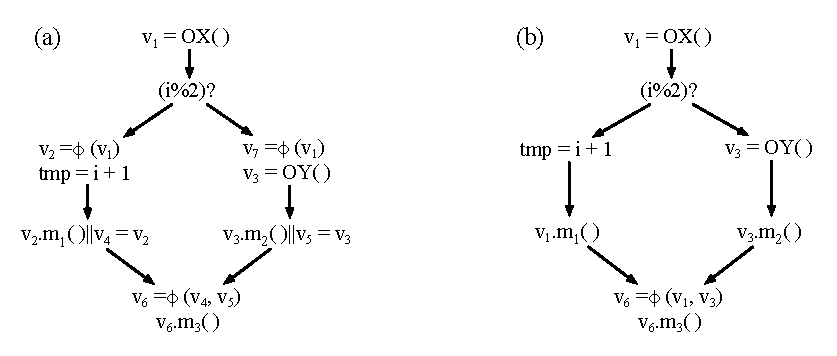
\includegraphics[scale=0.9]{sigImpl}
\caption{Implementing $\sigma$ functions via single arity $\phi$-functions.}
\label{fig:sigImpl}
\end{figure}

If $l$ is a branch point with $n$ successors that would contain a
$\sigma$-function $(v_1, \ldots, v_n) =\sigma v$, then, for each successor
$l_i$ of $l$, we insert at the beginning of $l_i$ an instruction
$v_i = \phi(v)$.
Notice that it is possible that $l_i$ already contains a $\phi$-function for
$v$.
This case happens when the control flow edge $l \rightarrow l_i$ is
{\em critical}.
A critical edge links a basic block with many successors to a basic block with
many predecessors.
If $l_i$ already contains a $\phi$-function $v' = \phi(\ldots, v, \ldots,)$,
then we rename $v$ to $v_i$.

\subsection{Deriving dense information from sparse analyses}
\label{sub:ssi:dense}

We can use our sparse dataflow analysis framework to solve even some dataflow
problems that demand information at every program point.
For instance, a well-known dataflow problem consists in determining the
bit-width of each integer variable in the program
code~\cite{Mahlke01,Stephenson00,Gawlitza09,Su04}.
This is a typical sparse analysis, for we are interested in collecting the
width, in bits, of each variable.
However, there exist clients of bit-width analyses that need to know the bit
sizes of the variables at particular program points.
For instance, Barik {\em et al.}~\cite{Barik06} have designed a bit-width
aware register allocator.
In this setting, the register pressure at a program point $p$ is the sum of
the bit sizes of all the variables alive at $p$.
The SSA graph can support the register allocator of Barik {\em et al.} by
coupling the result of the sparse bit-width analysis with live range information.
If the live range splitting strategy preserves the single static
assignment properties, then we can perform this coupling very efficiently.

Preserving the SSA properties is key due to two reasons.
First, liveness analysis has a non-iterative implementation for SSA form
programs that is linear on the program size~\cite[p.429]{Appel02}.
Second, and more important, in case we only need liveness information for some
specific variables, at some specific program points, there exist a fast
liveness check for SSA-form programs.
The problem of answering the question ``is variable $v$ alive at program point
$p$" has an algorithm that is $O(U)$, where $U$ is the number of times that $v$
is used in the program code~\cite{Benoit08}.
Given that the vast majority of variables in common benchmarks is used less
than 5 times~\cite{Benoit08}, we can consider this asymptotic complexity
constant in practice.